\begin{enumerate}[label=\thechapter.\arabic*,ref=\thechapter.\theenumi]
\item For the ordinary differential equation
\begin{align*}
\frac{d^3y}{dt^3} + 6\frac{d^2y}{dt^2} + 11\frac{dy}{dt} + 6y = 1,
\end{align*}
with initial conditions $y(0) = y'(0) = y''(0) = y'''(0) = 0$, the value of 
\begin{align*}
\lim_{{t \to \infty}} y(t) &= ?
\end{align*}
(round off to $3$ decimal places).
\hfill(GATE CH 2021)\\
\solution
\input{2021/CH/36/gate.tex}
\pagebreak
\item \textbf{Question:}
Consider the differential equation \\$\frac{d^2y}{dx^2}+8\frac{dy}{dx}+16y=0$ and the boundary conditions $y(0)=1$ and $\frac{dy}{dx}(0)=0$. The solution to equation is:\\
\hfill{(GATE.AE-1.2021)}\\
\solution
\input{2021/AE/1/gate3.tex}
\pagebreak
\item\textbf{Question:}
The solution of second-order differential equation \\ $\frac{d^2y}{dx^2}+2\frac{dy}{dx}+y=0$ with boundary conditions $y(0)=1$ and $y(1)=3$.\\
\hfill{(GATE  2021 CE.26)}\\
\solution
\input{2021/CE/26/gate4.tex}
\pagebreak
\item A system has a transfer function
\begin{align}
    G(s) = \frac{3e^{-4s}}{12s + 1}\nonumber
\end{align}
When a step-change of magnitude $M$ is given to the system input, the final value of the system output is measured to be 120. The value of M is \_\_\_\_\_.
\hfill(GATE 2021 CH Q52)\\
\solution
\input{2021/CH/52/GATE_CH_21_52.tex}
\pagebreak
\item The Bode magnitude plot for the transfer function $\frac{V_o(s)}{V_i(s)}$ of the circuit is as shown. The value of R is \_\_\_\_\_$\Omega$. \hfill(GATE 2021 EE Q20)
\begin{figure}[!ht]
    \centering
    \input{2021/EE/20/figs/tikz}
\end{figure}
\begin{figure}[!ht]
    \centering
    \includegraphics[width=\columnwidth]{2021/EE/20/figs/bode.png}
\end{figure}
\solution
\iffalse
\let\negmedspace\undefined
\let\negthickspace\undefined
\documentclass[journal,12pt,twocolumn]{IEEEtran}
\usepackage{cite}
\usepackage{amsmath,amssymb,amsfonts,amsthm}
\usepackage{algorithmic}
\usepackage{graphicx}
\usepackage{textcomp}
\usepackage{xcolor}
\usepackage{txfonts}
\usepackage{listings}
\usepackage{enumitem}
\usepackage{mathtools}
\usepackage{gensymb}
\usepackage{comment}
\usepackage[breaklinks=true]{hyperref}
\usepackage{tkz-euclide} 
\usepackage{listings}
\usepackage{gvv}                                        
\def\inputGnumericTable{}                                 
\usepackage[latin1]{inputenc}                                
\usepackage{color}                                            
\usepackage{array}                                            
\usepackage{longtable}                                       
\usepackage{calc}                                             
\usepackage{multirow}                                         
\usepackage{hhline}                                           
\usepackage{ifthen}                                           
\usepackage{lscape}
\usepackage[center]{caption} % center the captions to figure

\newtheorem{theorem}{Theorem}[section]
\newtheorem{problem}{Problem}
\newtheorem{proposition}{Proposition}[section]
\newtheorem{lemma}{Lemma}[section]
\newtheorem{corollary}[theorem]{Corollary}
\newtheorem{example}{Example}[section]
\newtheorem{definition}[problem]{Definition}
\newcommand{\BEQA}{\begin{eqnarray}}
\newcommand{\EEQA}{\end{eqnarray}}
\newcommand{\define}{\stackrel{\triangle}{=}}
\theoremstyle{remark}
\newtheorem{rem}{Remark}
\begin{document}

\newcolumntype{M}[1]{>{\centering\arraybackslash}m{#1}}
\newcolumntype{N}{@{}m{0pt}@{}}

\bibliographystyle{IEEEtran}
\vspace{3cm}

\title{GATE 2021 ME 3Q} 
\author{ee23btech11223 - Soham Prabhakar More% <-this % stops a space
}
\maketitle
\newpage
\bigskip

\renewcommand{\thefigure}{\theenumi}
\renewcommand{\thetable}{\theenumi}

\bibliographystyle{IEEEtran}

\textbf{Question:} The Dirac-delta function $\brak{\delta\brak{t - t_0}}$ for $t, t_0 \in \Re$, has the following property
\begin{align}
    \int_{a}^{b}\phi\brak{t}\delta\brak{t - t_0}dt = 
    \begin{cases}
        \phi\brak{t_0}\quad a < t_0 < b\\
        0 \quad\quad otherwise
    \end{cases} \label{eq:2022.ME.3.1}
\end{align}

The Laplace Transform of the Dirac-delta function $\delta\brak{t - a}$ for $a > 0; \mathcal{L}\brak{\delta\brak{t - a}} = F\brak{s}$ is

\hfill{(GATE 2021 ME 3Q)}

\solution
\fi
\begin{table}[ht]
    \renewcommand\thetable{1}
\begin{tabular}{|c|c|}
    \hline 
    \textbf{Parameter}&\textbf{Description} \\
    \hline
    $F\brak{s}$ & Laplace transform of $\delta\brak{t - a}$ \\
    \hline
    $G\brak{f}$ & Fourier transform of $\delta\brak{t - a}$ \\
    \hline
    $H\brak{t}$ & Fourier transform of a function with period $T$ \\
    \hline
    $w_T\brak{t}$ & Delta Comb, $\sum_{k = -\infty}^{\infty}\delta\brak{t - kT}$ \\
    \hline
    $W_T\brak{t}$ & Fourier transform of $w_T\brak{t}$ \\
    \hline
\end{tabular}

\caption{Table of parameters}
\label{Table:2022.ME.3.1}


\end{table} \\

By \eqref{eq:2022.ME.3.1} and $a > 0$,
\begin{align}
    F\brak{s} &= \int_{0}^{\infty}\delta\brak{t - a}e^{-st}dt \\
    \therefore F\brak{s} &= e^{-as}
\end{align}

The fourier transform,
\begin{align}
    G\brak{f} &= \int_{-\infty}^{\infty}\delta\brak{t - a}e^{-2\pi jft}dt \\
    \therefore G\brak{f} &= e^{-j2\pi fa}
\end{align}
For a periodic signal the fourier transform is defined as:
\begin{align}
    H\brak{f} &= \sum_{k = -\infty}^{\infty}c_k\delta\brak{f - \frac{k}{T}}
\end{align}
where $c_k$ are the fourier series coefficients and $T$ is the period. Thus,
\begin{align}
    W_T\brak{f} &= \sum_{k = -\infty}^{\infty}c_k\delta\brak{f - \frac{k}{T}} \\
    c_k &= \frac{1}{T}\int_{-\frac{T}{2}}^{\frac{T}{2}}w_T\brak{t}e^{-j2\pi \frac{k}{T}f}dt \\
    c_k &= \frac{1}{T}\int_{-\frac{T}{2}}^{\frac{T}{2}}\brak{\sum_{k = -\infty}^{\infty}\delta\brak{t - kT}}e^{-j2\pi \frac{k}{T}f}dt \\
\end{align}
\begin{align}
    c_k &= \frac{1}{T}\sum_{k = -\infty}^{\infty}\int_{-\frac{T}{2}}^{\frac{T}{2}}\delta\brak{t - kT}e^{-j2\pi \frac{k}{T}f}dt \\
    c_k &= \frac{1}{T} \\
    W_T\brak{f} &= \frac{1}{T}\sum_{k = -\infty}^{\infty}\delta\brak{f - \frac{k}{T}} \\
    \therefore W_T\brak{f} &= \frac{1}{T}w_{\frac{1}{T}}\brak{f}
\end{align}
Thus, the fourier transform of impulse train is another impulse train.
%\begin{align}
%    f\brak{t} &\system{F} H\brak{f} \\
%    f\brak{t + T} &\system{F} e^{j2\pi fT}H\brak{f} \\
%    \because e^{j2\pi fT}H\brak{f} &= H\brak{f} \\
%    H\brak{f}\brak{1 - e^{j2\pi fT}} &= 0
%\end{align}
%Thus, $H\brak{f}$ is zero everywhere except at $f = \frac{n}{T}, n \in Z$
%\begin{align}
%    \therefore H\brak{f} &= \sum_{k = -\infty}^{\infty}c_k\delta\brak{f - \frac{k}{T}} \\
%    \because \sum_{k = -\infty}^{\infty}c_ke^{-j2\pi f\frac{k}{T}} &\system{F} H\brak{f}
%\end{align}
%$c_k$ are the fourier series coefficents of $h\brak{t}$,
%\begin{align}
%    c_k = \int_{-\frac{T}{2}}^{\frac{T}{2}}
%\end{align}
%\end{document}

\pagebreak
\item Consider a system with transfer-function $G\brak{s}=\frac{2}{s+1}$. A unit-step function $\mu\brak{t}$ is applied to the system, which results in an output y\brak{t}. 

If $e\brak{t}=y\brak{t}-\mu\brak{t}$ then $ \lim_{t\to\infty} e(t)$ is\rule{1.5cm}{0.15mm}.
\solution
\iffalse
\let\negmedspace\undefined
\let\negthickspace\undefined
\documentclass[journal,12pt,twocolumn]{IEEEtran}
\usepackage{cite}
\usepackage{amsmath,amssymb,amsfonts,amsthm}
\usepackage{algorithmic}
\usepackage{graphicx}
\usepackage{textcomp}
\usepackage{xcolor}
\usepackage{txfonts}
\usepackage{listings}
\usepackage{enumitem}
\usepackage{mathtools}
\usepackage{gensymb}
\usepackage{comment}
\usepackage[breaklinks=true]{hyperref}
\usepackage{tkz-euclide} 
\usepackage{listings}
\usepackage{gvv}                                        
\def\inputGnumericTable{}                                 
\usepackage[latin1]{inputenc}                                
\usepackage{color}                                            
\usepackage{array}                                            
\usepackage{longtable}                                       
\usepackage{calc}                                             
\usepackage{multirow}                                         
\usepackage{hhline}                                           
\usepackage{ifthen}                                           
\usepackage{lscape}
\usepackage[center]{caption} % center the captions to figure

\newtheorem{theorem}{Theorem}[section]
\newtheorem{problem}{Problem}
\newtheorem{proposition}{Proposition}[section]
\newtheorem{lemma}{Lemma}[section]
\newtheorem{corollary}[theorem]{Corollary}
\newtheorem{example}{Example}[section]
\newtheorem{definition}[problem]{Definition}
\newcommand{\BEQA}{\begin{eqnarray}}
\newcommand{\EEQA}{\end{eqnarray}}
\newcommand{\define}{\stackrel{\triangle}{=}}
\theoremstyle{remark}
\newtheorem{rem}{Remark}
\begin{document}

\newcolumntype{M}[1]{>{\centering\arraybackslash}m{#1}}
\newcolumntype{N}{@{}m{0pt}@{}}

\bibliographystyle{IEEEtran}
\vspace{3cm}

\title{GATE 2021 ME 3Q} 
\author{ee23btech11223 - Soham Prabhakar More% <-this % stops a space
}
\maketitle
\newpage
\bigskip

\renewcommand{\thefigure}{\theenumi}
\renewcommand{\thetable}{\theenumi}

\bibliographystyle{IEEEtran}

\textbf{Question:} The Dirac-delta function $\brak{\delta\brak{t - t_0}}$ for $t, t_0 \in \Re$, has the following property
\begin{align}
    \int_{a}^{b}\phi\brak{t}\delta\brak{t - t_0}dt = 
    \begin{cases}
        \phi\brak{t_0}\quad a < t_0 < b\\
        0 \quad\quad otherwise
    \end{cases} \label{eq:2022.ME.3.1}
\end{align}

The Laplace Transform of the Dirac-delta function $\delta\brak{t - a}$ for $a > 0; \mathcal{L}\brak{\delta\brak{t - a}} = F\brak{s}$ is

\hfill{(GATE 2021 ME 3Q)}

\solution
\fi
\begin{table}[ht]
    \renewcommand\thetable{1}
\begin{tabular}{|c|c|}
    \hline 
    \textbf{Parameter}&\textbf{Description} \\
    \hline
    $F\brak{s}$ & Laplace transform of $\delta\brak{t - a}$ \\
    \hline
    $G\brak{f}$ & Fourier transform of $\delta\brak{t - a}$ \\
    \hline
    $H\brak{t}$ & Fourier transform of a function with period $T$ \\
    \hline
    $w_T\brak{t}$ & Delta Comb, $\sum_{k = -\infty}^{\infty}\delta\brak{t - kT}$ \\
    \hline
    $W_T\brak{t}$ & Fourier transform of $w_T\brak{t}$ \\
    \hline
\end{tabular}

\caption{Table of parameters}
\label{Table:2022.ME.3.1}


\end{table} \\

By \eqref{eq:2022.ME.3.1} and $a > 0$,
\begin{align}
    F\brak{s} &= \int_{0}^{\infty}\delta\brak{t - a}e^{-st}dt \\
    \therefore F\brak{s} &= e^{-as}
\end{align}

The fourier transform,
\begin{align}
    G\brak{f} &= \int_{-\infty}^{\infty}\delta\brak{t - a}e^{-2\pi jft}dt \\
    \therefore G\brak{f} &= e^{-j2\pi fa}
\end{align}
For a periodic signal the fourier transform is defined as:
\begin{align}
    H\brak{f} &= \sum_{k = -\infty}^{\infty}c_k\delta\brak{f - \frac{k}{T}}
\end{align}
where $c_k$ are the fourier series coefficients and $T$ is the period. Thus,
\begin{align}
    W_T\brak{f} &= \sum_{k = -\infty}^{\infty}c_k\delta\brak{f - \frac{k}{T}} \\
    c_k &= \frac{1}{T}\int_{-\frac{T}{2}}^{\frac{T}{2}}w_T\brak{t}e^{-j2\pi \frac{k}{T}f}dt \\
    c_k &= \frac{1}{T}\int_{-\frac{T}{2}}^{\frac{T}{2}}\brak{\sum_{k = -\infty}^{\infty}\delta\brak{t - kT}}e^{-j2\pi \frac{k}{T}f}dt \\
\end{align}
\begin{align}
    c_k &= \frac{1}{T}\sum_{k = -\infty}^{\infty}\int_{-\frac{T}{2}}^{\frac{T}{2}}\delta\brak{t - kT}e^{-j2\pi \frac{k}{T}f}dt \\
    c_k &= \frac{1}{T} \\
    W_T\brak{f} &= \frac{1}{T}\sum_{k = -\infty}^{\infty}\delta\brak{f - \frac{k}{T}} \\
    \therefore W_T\brak{f} &= \frac{1}{T}w_{\frac{1}{T}}\brak{f}
\end{align}
Thus, the fourier transform of impulse train is another impulse train.
%\begin{align}
%    f\brak{t} &\system{F} H\brak{f} \\
%    f\brak{t + T} &\system{F} e^{j2\pi fT}H\brak{f} \\
%    \because e^{j2\pi fT}H\brak{f} &= H\brak{f} \\
%    H\brak{f}\brak{1 - e^{j2\pi fT}} &= 0
%\end{align}
%Thus, $H\brak{f}$ is zero everywhere except at $f = \frac{n}{T}, n \in Z$
%\begin{align}
%    \therefore H\brak{f} &= \sum_{k = -\infty}^{\infty}c_k\delta\brak{f - \frac{k}{T}} \\
%    \because \sum_{k = -\infty}^{\infty}c_ke^{-j2\pi f\frac{k}{T}} &\system{F} H\brak{f}
%\end{align}
%$c_k$ are the fourier series coefficents of $h\brak{t}$,
%\begin{align}
%    c_k = \int_{-\frac{T}{2}}^{\frac{T}{2}}
%\end{align}
%\end{document}

\pagebreak
\item  Solution of differential equation $y'' + y'+ 0.25y = 0$ with initial values $y(0) = 3$ and $y'(0) = -3.5$ is
\begin{enumerate}
    \item[(A)] $ y = (3-2x)e^{0.5x} $
    \item[(B)] $ y = (3-2x)e^{-0.25x}$
    \item[(C)] $ y = (3-2x)e^{-0.5x}$
    \item[(D)] $ y = (2-3x)e^{-0.5x}$
\end{enumerate} 
\hfill(GATE AG 2021) \\
\solution
\iffalse
\let\negmedspace\undefined
\let\negthickspace\undefined
\documentclass[journal,12pt,twocolumn]{IEEEtran}
\usepackage{cite}
\usepackage{amsmath,amssymb,amsfonts,amsthm}
\usepackage{algorithmic}
\usepackage{graphicx}
\usepackage{textcomp}
\usepackage{xcolor}
\usepackage{txfonts}
\usepackage{listings}
\usepackage{enumitem}
\usepackage{mathtools}
\usepackage{gensymb}
\usepackage{comment}
\usepackage[breaklinks=true]{hyperref}
\usepackage{tkz-euclide} 
\usepackage{listings}
\usepackage{gvv}                                        
\def\inputGnumericTable{}                                 
\usepackage[latin1]{inputenc}                                
\usepackage{color}                                            
\usepackage{array}                                            
\usepackage{longtable}                                       
\usepackage{calc}                                             
\usepackage{multirow}                                         
\usepackage{hhline}                                           
\usepackage{ifthen}                                           
\usepackage{lscape}
\usepackage[center]{caption} % center the captions to figure

\newtheorem{theorem}{Theorem}[section]
\newtheorem{problem}{Problem}
\newtheorem{proposition}{Proposition}[section]
\newtheorem{lemma}{Lemma}[section]
\newtheorem{corollary}[theorem]{Corollary}
\newtheorem{example}{Example}[section]
\newtheorem{definition}[problem]{Definition}
\newcommand{\BEQA}{\begin{eqnarray}}
\newcommand{\EEQA}{\end{eqnarray}}
\newcommand{\define}{\stackrel{\triangle}{=}}
\theoremstyle{remark}
\newtheorem{rem}{Remark}
\begin{document}

\newcolumntype{M}[1]{>{\centering\arraybackslash}m{#1}}
\newcolumntype{N}{@{}m{0pt}@{}}

\bibliographystyle{IEEEtran}
\vspace{3cm}

\title{GATE 2021 ME 3Q} 
\author{ee23btech11223 - Soham Prabhakar More% <-this % stops a space
}
\maketitle
\newpage
\bigskip

\renewcommand{\thefigure}{\theenumi}
\renewcommand{\thetable}{\theenumi}

\bibliographystyle{IEEEtran}

\textbf{Question:} The Dirac-delta function $\brak{\delta\brak{t - t_0}}$ for $t, t_0 \in \Re$, has the following property
\begin{align}
    \int_{a}^{b}\phi\brak{t}\delta\brak{t - t_0}dt = 
    \begin{cases}
        \phi\brak{t_0}\quad a < t_0 < b\\
        0 \quad\quad otherwise
    \end{cases} \label{eq:2022.ME.3.1}
\end{align}

The Laplace Transform of the Dirac-delta function $\delta\brak{t - a}$ for $a > 0; \mathcal{L}\brak{\delta\brak{t - a}} = F\brak{s}$ is

\hfill{(GATE 2021 ME 3Q)}

\solution
\fi
\begin{table}[ht]
    \renewcommand\thetable{1}
\begin{tabular}{|c|c|}
    \hline 
    \textbf{Parameter}&\textbf{Description} \\
    \hline
    $F\brak{s}$ & Laplace transform of $\delta\brak{t - a}$ \\
    \hline
    $G\brak{f}$ & Fourier transform of $\delta\brak{t - a}$ \\
    \hline
    $H\brak{t}$ & Fourier transform of a function with period $T$ \\
    \hline
    $w_T\brak{t}$ & Delta Comb, $\sum_{k = -\infty}^{\infty}\delta\brak{t - kT}$ \\
    \hline
    $W_T\brak{t}$ & Fourier transform of $w_T\brak{t}$ \\
    \hline
\end{tabular}

\caption{Table of parameters}
\label{Table:2022.ME.3.1}


\end{table} \\

By \eqref{eq:2022.ME.3.1} and $a > 0$,
\begin{align}
    F\brak{s} &= \int_{0}^{\infty}\delta\brak{t - a}e^{-st}dt \\
    \therefore F\brak{s} &= e^{-as}
\end{align}

The fourier transform,
\begin{align}
    G\brak{f} &= \int_{-\infty}^{\infty}\delta\brak{t - a}e^{-2\pi jft}dt \\
    \therefore G\brak{f} &= e^{-j2\pi fa}
\end{align}
For a periodic signal the fourier transform is defined as:
\begin{align}
    H\brak{f} &= \sum_{k = -\infty}^{\infty}c_k\delta\brak{f - \frac{k}{T}}
\end{align}
where $c_k$ are the fourier series coefficients and $T$ is the period. Thus,
\begin{align}
    W_T\brak{f} &= \sum_{k = -\infty}^{\infty}c_k\delta\brak{f - \frac{k}{T}} \\
    c_k &= \frac{1}{T}\int_{-\frac{T}{2}}^{\frac{T}{2}}w_T\brak{t}e^{-j2\pi \frac{k}{T}f}dt \\
    c_k &= \frac{1}{T}\int_{-\frac{T}{2}}^{\frac{T}{2}}\brak{\sum_{k = -\infty}^{\infty}\delta\brak{t - kT}}e^{-j2\pi \frac{k}{T}f}dt \\
\end{align}
\begin{align}
    c_k &= \frac{1}{T}\sum_{k = -\infty}^{\infty}\int_{-\frac{T}{2}}^{\frac{T}{2}}\delta\brak{t - kT}e^{-j2\pi \frac{k}{T}f}dt \\
    c_k &= \frac{1}{T} \\
    W_T\brak{f} &= \frac{1}{T}\sum_{k = -\infty}^{\infty}\delta\brak{f - \frac{k}{T}} \\
    \therefore W_T\brak{f} &= \frac{1}{T}w_{\frac{1}{T}}\brak{f}
\end{align}
Thus, the fourier transform of impulse train is another impulse train.
%\begin{align}
%    f\brak{t} &\system{F} H\brak{f} \\
%    f\brak{t + T} &\system{F} e^{j2\pi fT}H\brak{f} \\
%    \because e^{j2\pi fT}H\brak{f} &= H\brak{f} \\
%    H\brak{f}\brak{1 - e^{j2\pi fT}} &= 0
%\end{align}
%Thus, $H\brak{f}$ is zero everywhere except at $f = \frac{n}{T}, n \in Z$
%\begin{align}
%    \therefore H\brak{f} &= \sum_{k = -\infty}^{\infty}c_k\delta\brak{f - \frac{k}{T}} \\
%    \because \sum_{k = -\infty}^{\infty}c_ke^{-j2\pi f\frac{k}{T}} &\system{F} H\brak{f}
%\end{align}
%$c_k$ are the fourier series coefficents of $h\brak{t}$,
%\begin{align}
%    c_k = \int_{-\frac{T}{2}}^{\frac{T}{2}}
%\end{align}
%\end{document}

\pagebreak
\item Consider the following first order partial differential equation, also known as the transport equation
\begin{align*}
\frac{\partial y\brak{x,t}}{\partial t}+5\frac{\partial y\brak{x,t}}{\partial x}&=0
\end{align*}
with initial conditions given by $y(x, 0) = \sin x,-\infty < x < \infty$. The value of $y(x, t)$ at $x = \pi$ and $t=\frac{\pi}{6}$ is  \rule{1cm}{0.15mm}.
\begin{enumerate}[label=(\Alph*)]
\item 1
\item 2
\item 0
\item 0.5
\end{enumerate}
\hfill(GATE 2021 BM Q28)\\
\solution
\input{2021/BM/28/28.tex}
\pagebreak
\item In the circuit, switch 'S' is in the closed position for a very long time. If the switch is opened at time $t=0$, then $i_L\brak{t}$ in amperes, for $t\geq0$ is
\input{2021/EE/29/figs/fig_1}\\
\hfill(GATE 2021 EE 29)\\
\solution
\iffalse
\let\negmedspace\undefined
\let\negthickspace\undefined
\documentclass[journal,12pt,twocolumn]{IEEEtran}
\usepackage{cite}
\usepackage{amsmath,amssymb,amsfonts,amsthm}
\usepackage{algorithmic}
\usepackage{graphicx}
\usepackage{textcomp}
\usepackage{xcolor}
\usepackage{txfonts}
\usepackage{listings}
\usepackage{enumitem}
\usepackage{mathtools}
\usepackage{gensymb}
\usepackage{comment}
\usepackage[breaklinks=true]{hyperref}
\usepackage{tkz-euclide} 
\usepackage{listings}
\usepackage{gvv}                                        
\def\inputGnumericTable{}                                 
\usepackage[latin1]{inputenc}                                
\usepackage{color}                                            
\usepackage{array}                                            
\usepackage{longtable}                                       
\usepackage{calc}                                             
\usepackage{multirow}                                         
\usepackage{hhline}                                           
\usepackage{ifthen}                                           
\usepackage{lscape}
\usepackage[center]{caption} % center the captions to figure

\newtheorem{theorem}{Theorem}[section]
\newtheorem{problem}{Problem}
\newtheorem{proposition}{Proposition}[section]
\newtheorem{lemma}{Lemma}[section]
\newtheorem{corollary}[theorem]{Corollary}
\newtheorem{example}{Example}[section]
\newtheorem{definition}[problem]{Definition}
\newcommand{\BEQA}{\begin{eqnarray}}
\newcommand{\EEQA}{\end{eqnarray}}
\newcommand{\define}{\stackrel{\triangle}{=}}
\theoremstyle{remark}
\newtheorem{rem}{Remark}
\begin{document}

\newcolumntype{M}[1]{>{\centering\arraybackslash}m{#1}}
\newcolumntype{N}{@{}m{0pt}@{}}

\bibliographystyle{IEEEtran}
\vspace{3cm}

\title{GATE 2021 ME 3Q} 
\author{ee23btech11223 - Soham Prabhakar More% <-this % stops a space
}
\maketitle
\newpage
\bigskip

\renewcommand{\thefigure}{\theenumi}
\renewcommand{\thetable}{\theenumi}

\bibliographystyle{IEEEtran}

\textbf{Question:} The Dirac-delta function $\brak{\delta\brak{t - t_0}}$ for $t, t_0 \in \Re$, has the following property
\begin{align}
    \int_{a}^{b}\phi\brak{t}\delta\brak{t - t_0}dt = 
    \begin{cases}
        \phi\brak{t_0}\quad a < t_0 < b\\
        0 \quad\quad otherwise
    \end{cases} \label{eq:2022.ME.3.1}
\end{align}

The Laplace Transform of the Dirac-delta function $\delta\brak{t - a}$ for $a > 0; \mathcal{L}\brak{\delta\brak{t - a}} = F\brak{s}$ is

\hfill{(GATE 2021 ME 3Q)}

\solution
\fi
\begin{table}[ht]
    \renewcommand\thetable{1}
\begin{tabular}{|c|c|}
    \hline 
    \textbf{Parameter}&\textbf{Description} \\
    \hline
    $F\brak{s}$ & Laplace transform of $\delta\brak{t - a}$ \\
    \hline
    $G\brak{f}$ & Fourier transform of $\delta\brak{t - a}$ \\
    \hline
    $H\brak{t}$ & Fourier transform of a function with period $T$ \\
    \hline
    $w_T\brak{t}$ & Delta Comb, $\sum_{k = -\infty}^{\infty}\delta\brak{t - kT}$ \\
    \hline
    $W_T\brak{t}$ & Fourier transform of $w_T\brak{t}$ \\
    \hline
\end{tabular}

\caption{Table of parameters}
\label{Table:2022.ME.3.1}


\end{table} \\

By \eqref{eq:2022.ME.3.1} and $a > 0$,
\begin{align}
    F\brak{s} &= \int_{0}^{\infty}\delta\brak{t - a}e^{-st}dt \\
    \therefore F\brak{s} &= e^{-as}
\end{align}

The fourier transform,
\begin{align}
    G\brak{f} &= \int_{-\infty}^{\infty}\delta\brak{t - a}e^{-2\pi jft}dt \\
    \therefore G\brak{f} &= e^{-j2\pi fa}
\end{align}
For a periodic signal the fourier transform is defined as:
\begin{align}
    H\brak{f} &= \sum_{k = -\infty}^{\infty}c_k\delta\brak{f - \frac{k}{T}}
\end{align}
where $c_k$ are the fourier series coefficients and $T$ is the period. Thus,
\begin{align}
    W_T\brak{f} &= \sum_{k = -\infty}^{\infty}c_k\delta\brak{f - \frac{k}{T}} \\
    c_k &= \frac{1}{T}\int_{-\frac{T}{2}}^{\frac{T}{2}}w_T\brak{t}e^{-j2\pi \frac{k}{T}f}dt \\
    c_k &= \frac{1}{T}\int_{-\frac{T}{2}}^{\frac{T}{2}}\brak{\sum_{k = -\infty}^{\infty}\delta\brak{t - kT}}e^{-j2\pi \frac{k}{T}f}dt \\
\end{align}
\begin{align}
    c_k &= \frac{1}{T}\sum_{k = -\infty}^{\infty}\int_{-\frac{T}{2}}^{\frac{T}{2}}\delta\brak{t - kT}e^{-j2\pi \frac{k}{T}f}dt \\
    c_k &= \frac{1}{T} \\
    W_T\brak{f} &= \frac{1}{T}\sum_{k = -\infty}^{\infty}\delta\brak{f - \frac{k}{T}} \\
    \therefore W_T\brak{f} &= \frac{1}{T}w_{\frac{1}{T}}\brak{f}
\end{align}
Thus, the fourier transform of impulse train is another impulse train.
%\begin{align}
%    f\brak{t} &\system{F} H\brak{f} \\
%    f\brak{t + T} &\system{F} e^{j2\pi fT}H\brak{f} \\
%    \because e^{j2\pi fT}H\brak{f} &= H\brak{f} \\
%    H\brak{f}\brak{1 - e^{j2\pi fT}} &= 0
%\end{align}
%Thus, $H\brak{f}$ is zero everywhere except at $f = \frac{n}{T}, n \in Z$
%\begin{align}
%    \therefore H\brak{f} &= \sum_{k = -\infty}^{\infty}c_k\delta\brak{f - \frac{k}{T}} \\
%    \because \sum_{k = -\infty}^{\infty}c_ke^{-j2\pi f\frac{k}{T}} &\system{F} H\brak{f}
%\end{align}
%$c_k$ are the fourier series coefficents of $h\brak{t}$,
%\begin{align}
%    c_k = \int_{-\frac{T}{2}}^{\frac{T}{2}}
%\end{align}
%\end{document}

\pagebreak
\item Let $ u(t) $ denote the unit step function . The bilateral laplace transform function  $ f(t) = e^t u(-t) $ is 
\begin{enumerate}
\item[A] $ \frac{1}{s-1}$ with real part of $ s> 1$
\item[B]$\frac{-1}{s-1}$ with real part of $ s> 1$
\item[C]$\frac{1}{s-1}$ with real part of $ s< 1$
\item[D]$\frac{-1}{s-1}$ with real part of $ s< 1$
\end{enumerate}
\hfill (GATE 2021 IN) \\
\solution
\input{2021/IN/6/in06.tex}

\item Given $y(t) = e^{-3t}u(t) * u(t+3)$, where * denotes convolution operation. The value of $y(t)$ as $t \rightarrow \infty$ is
\hfill{(GATE IN 2021)}\\
\solution
\iffalse
\let\negmedspace\undefined
\let\negthickspace\undefined
\documentclass[journal,12pt,twocolumn]{IEEEtran}
\usepackage{cite}
\usepackage{amsmath,amssymb,amsfonts,amsthm}
\usepackage{algorithmic}
\usepackage{graphicx}
\usepackage{textcomp}
\usepackage{xcolor}
\usepackage{txfonts}
\usepackage{listings}
\usepackage{enumitem}
\usepackage{mathtools}
\usepackage{gensymb}
\usepackage{comment}
\usepackage[breaklinks=true]{hyperref}
\usepackage{tkz-euclide}
\usepackage{listings}
\usepackage{gvv}
\def\inputGnumericTable{}
\usepackage[latin1]{inputenc}
\usepackage{color}
\usepackage{array}
\usepackage{longtable}
\usepackage{calc}
\usepackage{multirow}
\usepackage{hhline}
\usepackage{ifthen}
\usepackage{lscape}
\usepackage{circuitikz}

\newtheorem{theorem}{Theorem}[section]
\newtheorem{problem}{Problem}
\newtheorem{proposition}{Proposition}[section]
\newtheorem{lemma}{Lemma}[section]
\newtheorem{corollary}[theorem]{Corollary}
\newtheorem{example}{Example}[section]
\newtheorem{definition}[problem]{Definition}
\newcommand{\BEQA}{\begin{eqnarray}}
\newcommand{\EEQA}{\end{eqnarray}}
\newcommand{\define}{\stackrel{\triangle}{=}}
\theoremstyle{remark}
\newtheorem{rem}{Remark}
\begin{document}

\bibliographystyle{IEEEtran}
\vspace{3cm}

\title{Gate 2021- Instrumentation Engineering}
\author{EE23BTECH11058 - Sindam Ananya$^{*}$% <-this % stops a space
}
\maketitle
\newpage
\bigskip

\renewcommand{\thefigure}{\theenumi}
\renewcommand{\thetable}{\theenumi}

\vspace{3cm}
\textbf{Question 43:} 
Given $y(t) = e^{-3t}u(t) * u(t+3)$, where * denotes convolution operation. The value of $y(t)$ as $t \rightarrow \infty$ is
\hfill{(GATE IN 2021)}\\
\solution
\fi
\begin{align}
y(t) &=  e^{-3t}u(t) * u(t+3)\\
x(t) &\xleftrightarrow{\mathcal{L}} X(s)\\
x(t-t_o) &\xleftrightarrow{\mathcal{L}} e^{-s t_o}X(s)\\
x_1(t) * x_2(t) &\xleftrightarrow{\mathcal{L}} X_1(s)X_2(s)\\
e^{-at}u(t) &\xleftrightarrow{\mathcal{L}} \frac{1}{s + a} \quad \brak{ROC:Re(s)>-a}\\
u(t) &\xleftrightarrow{\mathcal{L}} \frac{1}{s} \quad \brak{ROC:Re(s)>0}\\
u(t+3) &\xleftrightarrow{\mathcal{L}} \frac{e^{3s}}{s} \quad \brak{ROC:Re(s)>0}\\ 
Y(s) &= \brak{\frac{1}{s + 3}}\brak{\frac{e^{3s}}{s}} \quad \brak{ROC:Re(s)>0}
\label{eq:gate202143}
\end{align}
By using Final Value Theorem,
\begin{align}
\lim\limits_{t \to \infty} y(t) &= \lim\limits_{s \to 0} sY(s)\\
                                &= \lim\limits_{s \to 0} s\brak{\frac{1}{s + 3}}\brak{\frac{e^{3s}}{s}}\\
                                &= \frac{1}{3}
\end{align}
By solving the equation \eqref{eq:gate202143} through partial fractions,
\begin{align}
Y(s) = \frac{e^{3s}}{3s} - \frac{e^{3s}}{3\brak{s+3}} 
\end{align}
By applying inverse laplace transform,
\begin{align}
y(t) = \frac{u(t+3)}{3} - \frac{e^{-3(t+3)}u(t+3)}{3}
\end{align}
\begin{figure}[h!]
    \centering
    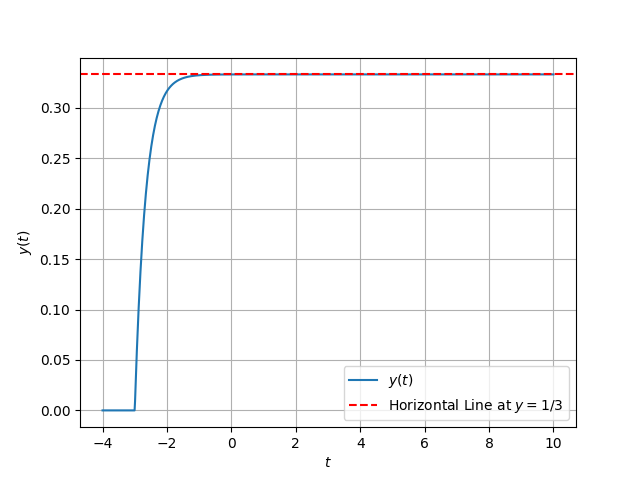
\includegraphics[width=0.8\columnwidth]{2021/IN/43/figs/plot.png}
    \caption{plot of $y(t)$}
    \label{fig:gate202138fig}
\end{figure}
%\end{document}

\pagebreak

\end{enumerate}
